% Uncomment this to make slides with overlays:
%\documentclass[slides]{beamer}

% Uncomment these (but comment the above \documentclass line) to make handouts:
\documentclass[handout]{beamer}

% Uncomment these to have more than one slide per page
\usepackage{pgfpages}
\pgfpagesuselayout{2 on 1}[border shrink=5mm]
\pgfpageslogicalpageoptions{1}{border code=\pgfusepath{stroke}}
\pgfpageslogicalpageoptions{2}{border code=\pgfusepath{stroke}}

\usepackage[]{graphicx, color, hyperref}

\mode<presentation>
{
	%\usetheme[secheader]{Boadilla}
	%\usecolortheme[rgb={.835, .102,.169}]{structure}  
	\usetheme[width= 0cm]{Goettingen}
	%\setbeamercovered{transparent}
}
\setbeamertemplate{navigation symbols}{}
\setbeamertemplate{footline}[frame number]

\definecolor{blue2}{rgb}{0.278,0.278,0.729} 
\newcommand{\blue}[1]{\textcolor{blue2}{#1}}
\newcommand{\white}[1]{\textcolor{white}{#1}}
\newcommand{\red}[1]{\textcolor{red}{#1}}
\newcommand{\xbar}{\overline{x}}
\newcommand{\ybar}{\overline{y}}
\newcommand{\phat}{\widehat{p}}
\newcommand{\prob}{\mbox{Pr}}
\newcommand{\E}{\mathbb{E}}
\newcommand{\Var}{\mbox{Var}}
\newcommand{\cp}{\oplus}
\newcommand{\cm}{\circleddash}

\title{Lecture 10: Bernoulli and Geometric Random Variables}
\author{Chapter 3.3-3.5}
\date{}


\begin{document}
%------------------------------------------------------------------------------
\begin{frame}
\titlepage
\end{frame}
%------------------------------------------------------------------------------



%------------------------------------------------------------------------------
\begin{frame}[fragile]
\frametitle{Goals for Today}

Define
\begin{itemize}
\item Bernoulli random variables
\item Geometric random variables
\end{itemize}


\end{frame}
%------------------------------------------------------------------------------


%------------------------------------------------------------------------------
\begin{frame}[fragile]
\frametitle{Mathematical Definition of a Bernoulli Random Variable}

A \blue{random variable $X$} is a random process or variable with a numerical outcome.  

\vspace{5cm}

\pause Random variables are described in terms of their \blue{distribution}.
\end{frame}
%------------------------------------------------------------------------------


%------------------------------------------------------------------------------
\begin{frame}
\frametitle{Bernoulli Distribution}
Say we have an experiment where we define each \blue{trial} (or instance) to have two possible outcomes of interest.  Examples
\pause\begin{itemize}
\item Coin flips:  heads vs tails
\item Medical test (for a disease):  positive vs negative
\item Rolling a die and getting a 6 vs not getting a 6
\end{itemize}

\vspace{0.5cm}

\pause In each case we can \blue{define} the outcomes to be \blue{success} vs \blue{failure}.  No moral judgement; just labels.

\end{frame}
%------------------------------------------------------------------------------


%------------------------------------------------------------------------------
\begin{frame}
\frametitle{Bernoulli Distribution}

Say we have trials where we have two outcomes:  either a ``success'' or a ``failure''.  Classic example:  coin flips have $p=0.5$ of heads, if we define heads as the success.

\vspace{0.5cm}

\begin{itemize}
\item probability $p$ of a ``success.''  Denote successes with a ``1.''
\item probability $1-p$ of a ``failure.''  Denote failures with a ``0.''
\end{itemize}


\end{frame}
%------------------------------------------------------------------------------


%------------------------------------------------------------------------------
\begin{frame}[fragile]
\frametitle{Definition of a Bernoulli Random Variable}

If $X$ is a random variable that takes value
\begin{itemize}
\item 1 with probability of success $p$
\item 0 with probability of failure $1-p$
\end{itemize}

then $X$ is a \blue{Bernoulli random variable} with mean and standard deviation:
\begin{eqnarray*}
\mu &=& p\\
\sigma &=& \sqrt{p(1-p)}
\end{eqnarray*}

\end{frame}
%------------------------------------------------------------------------------


%------------------------------------------------------------------------------
\begin{frame}[fragile]
\frametitle{Intuition Behind $\sigma$}


\end{frame}
%------------------------------------------------------------------------------


%------------------------------------------------------------------------------
\begin{frame}[fragile]
\frametitle{Sample Proportion}
Say you repeat $n$ instances of a Bernoulli random variable.  You end up with a sample $x_1, \ldots, x_{n}$

\vspace{0.5cm}

The \blue{sample proportion $\widehat{p}$} (p-hat) is the sample mean of these observations.  i.e. \[
\widehat{p} = \frac{\mbox{\# of successes}}{\mbox{\# of trials}} = \frac{1}{n}\sum_{i=1}^{n}x_i
\]

\end{frame}
%------------------------------------------------------------------------------


%------------------------------------------------------------------------------
\begin{frame}[fragile]
\frametitle{Example of Bernoulli Distribution}

\begin{itemize}
\pause\item A success as rolling a 6.\\
So $P(X=1) = P(\mbox{success}) = p =  \frac{1}{6}$.
\pause\item A failure as rolling anything else.\\
So $P(X=0) = P(\mbox{failure}) = 1-p = \frac{5}{6}$.
\end{itemize}

\end{frame}
%------------------------------------------------------------------------------


%------------------------------------------------------------------------------
\begin{frame}[fragile]
\frametitle{Back to Lecture 3.1: Population vs Sample Values}

\begin{center}
  \begin{tabular}{r|cc}
	\hline	
     & True Population Value & Sample Value \\ 
	\hline	
    Mean & $\mu$ & $\overline{x}$ \\ 
    Variance & $\sigma^2$ & $s^2$ \\ 
    Standard Deviation & $\sigma$ & $s$ \\ 
    \blue{Proportion} & \blue{$p$} & \blue{$\widehat{p}$} \\
	\hline	
  \end{tabular}
\end{center}

\vspace{0.5cm}

\pause The \blue{sample proportion $\widehat{p}$} is a specific kind of \blue{sample mean} for Bernoulli random variables, which \blue{estimates $p$}, a specific kind of population mean.  

\end{frame}
%------------------------------------------------------------------------------


%------------------------------------------------------------------------------
\begin{frame}[fragile]
\frametitle{Scenario}

\blue{Question}:  Say
\begin{itemize}
\item the San Francisco Giants have equal probability $p=0.6$ of winning any game
\item games are independent
\end{itemize}

It's the beginning of the season.  What is the probability that they don't win their first game until the 5th game of the season?

\vspace{0.5cm}

\pause For this to happen, there must be 4 loses in the first 4 games AND a win in the 5th game:
\begin{eqnarray*}
P(\mbox{1st W in 5th game}) &=& P(\mbox{4 loses}) \times P(\mbox{win})\\
&=& (P(\mbox{loss}))^4 \times P(\mbox{win})\\
&=& (1-p)^4 \times p\\
&=& 0.4^4 \times 0.6 = 0.01536.
\end{eqnarray*}


\end{frame}
%------------------------------------------------------------------------------	


%------------------------------------------------------------------------------
\begin{frame}[fragile]
\frametitle{Geometric Random Variables}

\blue{Geometric Distribution}: If the probability of a success in any trial is $p$, the trials are independent,
then the probability of finding the first success on the $n^{\mbox{th}}$ trial is given by
\[
(1-p)^{n-1}p
\]

\pause Also
\begin{eqnarray*}
\mu &=& \frac{1}{p}\\
\sigma^2 &=& \frac{1-p}{p^2}\\
\sigma &=& \frac{\sqrt{1-p}}{p}
\end{eqnarray*}


\end{frame}
%------------------------------------------------------------------------------	


%------------------------------------------------------------------------------
\begin{frame}[fragile]
\frametitle{Intuition Behind $\mu$}

Think about $\mu$:  $\frac{1}{p}$ is the average number of trials we need until the \blue{first} success.

\vspace{0.5cm}

\pause So compare:
\begin{itemize}
\item Say $p=0.5$.  Then $\mu = \frac{1}{0.5} = 2$
\item Say $p=0.001$.  Then $\mu = \frac{1}{0.001} = 1000$
\end{itemize}

\vspace{0.5cm}

\pause In the first case, the probability of a success is \blue{lower}, so we expect on average it will take more trials until the \blue{first} success.  

\end{frame}
%------------------------------------------------------------------------------	


%------------------------------------------------------------------------------
\begin{frame}[fragile]
\frametitle{Yesterday's Quiz: Placebos}

\blue{Question 1}: Was Dr. Irving Kirsch arguing that anti-depressants are no better than placebos for everyone with depression?

\vspace{0.5cm}

\pause\blue{Solution}: No, while he argued that anti-depressants were no better than placebo for those with mild to moderate depression, he is of the opinion that there is clinical benefit for those who are severely depressed.  


\end{frame}
%------------------------------------------------------------------------------	


%------------------------------------------------------------------------------
\begin{frame}[fragile]
\frametitle{Yesterday's Quiz: Placebos}
\blue{Question 2}: What is Dr. Walter Brown's (bald guy from Yale) criticism of the way the FDA approves anti-depressants?

\vspace{0.5cm}

\pause\blue{Solution}:  That all that is required are two clinical trials where the drug performs better than placebo, regardless of the number of trials with ``negative results.''  Ex:  say a drug performs better than placebo in 2 trials, but fails in 998 trials, it will still be approved by the FDA.  

\end{frame}
%------------------------------------------------------------------------------	


%%------------------------------------------------------------------------------
%\begin{frame}
%\frametitle{Binomial Distribution}
%
%So say now, instead of $P(\mbox{1st W in 5th game}) = P(\mbox{\blue{LLLLW}})$, we want the probability that they win \blue{exactly one} out of the five games.  Five ways:
%
%\pause\begin{center}
%\begin{tabular}{c|ll}
%Pattern & Probability & Equals\\
%\hline
%\blue{WLLLL} & $p \times (1-p)^4$ & $=p\times(1-p)^4$\\
%\blue{LWLLL} & $(1-p) \times p \times (1-p)^3$ & $=p\times(1-p)^4$\\
%\blue{LLWLL} & $(1-p)^2 \times p \times (1-p)^2$& $=p\times(1-p)^4$\\
%\blue{LLLWL} & $(1-p)^3 \times p \times (1-p)$& $=p\times(1-p)^4$\\
%\blue{LLLLW} & $(1-p)^4 \times p$& $=p\times(1-p)^4$\\
%\end{tabular} 
%\end{center}
%
%\pause Each pattern (book calls it scenario) has the same probability regardless of order by independence, and there are 5 ways to \blue{choose} the pattern.
%
%\vspace{0.25cm}
%
%\pause So $P(\mbox{win exactly one out of five})$ is  $5 \times p\times(1-p)^4 = 5 \times 0.4^4 \times 0.6 = 0.0768$
%
%\end{frame}
%%------------------------------------------------------------------------------
%
%
%
%%------------------------------------------------------------------------------
%\begin{frame}
%\frametitle{Step Back... Example of $n$ choose $k$}
%Say I give you $n=5$ balls labeled 1 thru 5.  How many different ways can you choose $k=3$ of them?
%
%\begin{center}
%\pause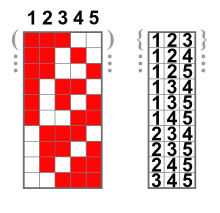
\includegraphics[height=4cm]{figure/choose.png}
%\end{center}
%
%As we see, 10 ways.  
%
%\end{frame}
%%------------------------------------------------------------------------------
%
%
%
%%------------------------------------------------------------------------------
%\begin{frame}
%\frametitle{Step Back... $n$ choose $k$ in General}
%Say I give you $n$ balls labeled 1 thru n.  How many different ways can you choose $k$ of them?
%
%\[
%{n \choose k} = \frac{n!}{k!(n-k)!}
%\]
%
%This is read \blue{n choose k}.  
%
%\pause \vspace{0.5cm}
%
%In example: $n=5$ and $k=3$
%\[
%{5 \choose 3} = \frac{5!}{3!(5-3)!} = \frac{5 \times 4 \times 3 \times 2 \times 1}{(3 \times 2 \times 1)(2 \times 1)} = \frac{120}{12} = 10
%\]
%
%Note that $0!=1$
%
%\end{frame}
%%------------------------------------------------------------------------------
%
%
%%------------------------------------------------------------------------------
%\begin{frame}
%\frametitle{Binomial Distribution}
%Suppose the probability of a single trial being a success is $p$.  Then the probability of observing exactly $k$ successes in $n$ independent trials is given by:
%
%\pause\begin{eqnarray*}
%P(\mbox{exactly $k$ successes}) &=& {n \choose k} p^k (1-p)^{n-k}\\
%&=& \frac{n!}{k!(n-k)!}p^k (1-p)^{n-k}
%\end{eqnarray*}
%
%\pause The mean, variance, and SD are:
%\[
%\mu = np \hspace{1cm} \sigma^2 = np(1-p) \hspace{1cm} \sigma = \sqrt{np(1-p)}
%\]
%
%\end{frame}
%%------------------------------------------------------------------------------
%
%
%%------------------------------------------------------------------------------
%\begin{frame}
%\frametitle{Conditions for Binomial Distribution}
%
%\begin{enumerate}
%\pause\item The trials are independent.
%\pause\item The number of trials $n$ is fixed
%\pause\item Each trial outcome can be classified as a failure or a success
%\pause\item The probability of a success $p$ is the same for each trial
%\end{enumerate}
%
%\end{frame}
%%------------------------------------------------------------------------------
%
%
%%------------------------------------------------------------------------------
%\begin{frame}
%\frametitle{Back to Soccer Example}
%The Portland Timbers have equal probability p = 0.6 of winning any particular soccer game. We want the probability that they win \blue{exactly one} out of the five games.  Five ways:
%
%\pause\begin{center}
%\begin{tabular}{c|ll}
%Pattern & Probability & Equals\\
%\hline
%\blue{WLLLL} & $p \times (1-p)^4$ & $=p\times(1-p)^4$\\
%\blue{LWLLL} & $(1-p) \times p \times (1-p)^3$ & $=p\times(1-p)^4$\\
%\blue{LLWLL} & $(1-p)^2 \times p \times (1-p)^2$& $=p\times(1-p)^4$\\
%\blue{LLLWL} & $(1-p)^3 \times p \times (1-p)$& $=p\times(1-p)^4$\\
%\blue{LLLLW} & $(1-p)^4 \times p$& $=p\times(1-p)^4$\\
%\end{tabular} 
%\end{center}
%
%\pause Letting a win be a ``success'':
%\begin{eqnarray*}
%P(\mbox{$k=1$ win}) &=& {n \choose k} p^k (1-p)^{n-k} = \frac{5!}{1!\times4!} 0.6 \times 0.4^4\\
%&=& 5 \times  0.6 \times 0.4^4 = 0.0768
%\end{eqnarray*}
%
%\end{frame}
%%------------------------------------------------------------------------------
%
%
%%------------------------------------------------------------------------------
%\begin{frame}
%\frametitle{Back to Soccer Example}
%What about the probability that they win all their games!  i.e. $k=5$:
%\pause \begin{eqnarray*}
%P(\mbox{$k=5$ wins}) &=& {n \choose k} p^k (1-p)^{n-k} = {5 \choose 5} 0.6^5 (1-0.6)^{0}\\
%&=& \frac{5!}{5!\times 0!} 0.6^5 \times 1 = 0.08
%\end{eqnarray*}
%
%\vspace{0.75cm}
%
%\pause What about the probability that they at win at least one game?
%\pause \begin{eqnarray*}
%P(\mbox{at least $k=1$ wins}) &=& P(\mbox{$k=1$ win}) + \ldots + P(\mbox{$k=5$ wins}) \\
%&=& 1 - P(\mbox{k=0 wins})\\
%&=& 1 -  \frac{5!}{0!\times 5!} 0.6^0 \times 0.4^5 = 1 - 0.01024\\
%&=& 0.98976
%\end{eqnarray*}
%
%
%\end{frame}
%%------------------------------------------------------------------------------
%
%
%%pdf("./5.1 Binomial+Poisson/bin.pdf", width=7, height=5)
%%x <- c(0:5)
%%y <- dbinom(x, size=5, prob=0.6)
%%plot(x,y, xlab="k: number of successes", ylab="P(k successes)", ylim=c(0, max(y)))
%%points(x,y, pch=19, cex=1.5)
%%dev.off()
%%------------------------------------------------------------------------------
%\begin{frame}
%\frametitle{Back to Soccer Example}
%
%\begin{center}
%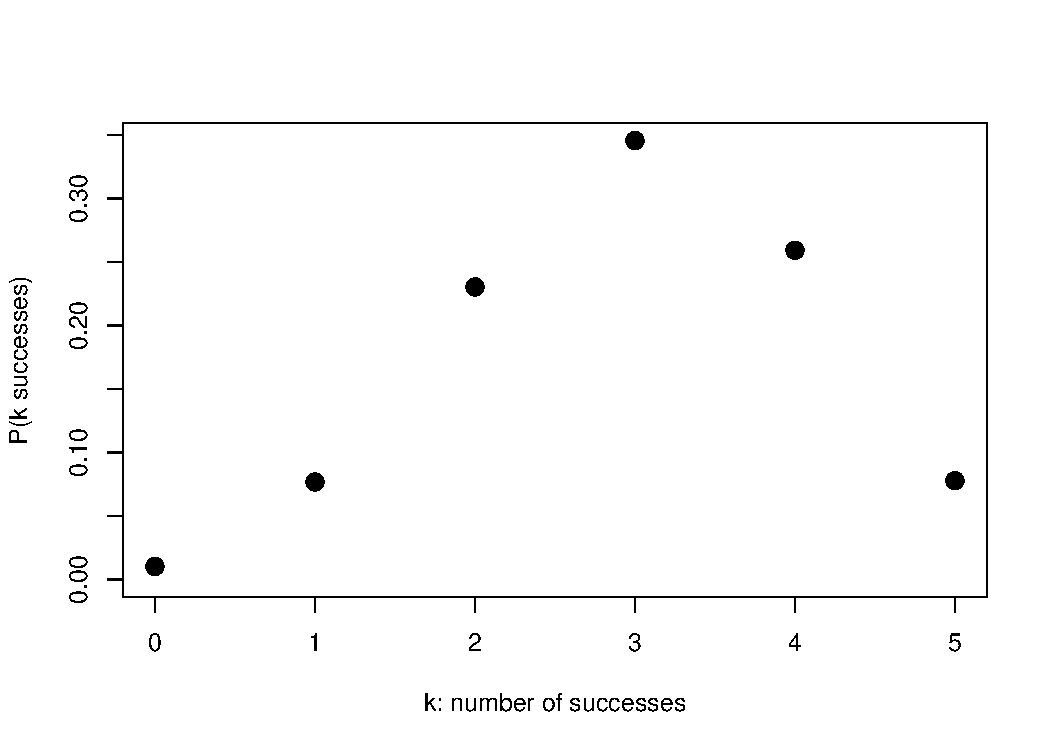
\includegraphics[width=8cm]{figure/bin.pdf}
%\end{center}
%
%\end{frame}
%%------------------------------------------------------------------------------
%
%
%%------------------------------------------------------------------------------
%\begin{frame}
%\frametitle{Poisson Distribution}
%
%Say you want to count the number of rare events in a large population over a unit of time.  Examples:
%\begin{itemize}
%\pause \item the number of car accidents at a particular intersection on a given week
%\pause \item the number of ambulance calls on any given day in Portland
%\pause \item the number of soldiers in the Prussian army killed accidentally by horse kick from 1875 to 1894
%\end{itemize}
%
%\vskip 0.25cm
%
%\pause The \blue{Poisson distribution} helps us describe the number of such events that will occur in a short unit of time for a fixed population if the individuals within the population are
%independent.
%
%\end{frame}
%%------------------------------------------------------------------------------
%
%
%%------------------------------------------------------------------------------
%\begin{frame}
%\frametitle{Poisson Distribution}
%Suppose we are watching for rare events and the number of observed events follows a Poisson distribution with rate $\lambda$
%\[
%    P(\mbox{observe k rare events}) = \frac{\lambda^k e^{-\lambda}}{k!}
%\]
%\pause where k may take a value 0, 1, 2, \ldots where $e \approx 2.718$.
%
%\vspace{0.5cm}
%
%\pause The mean and SD are $\lambda$ and $\sqrt{\lambda}$.
%
%\end{frame}
%%------------------------------------------------------------------------------
%
%
%%------------------------------------------------------------------------------
%\begin{frame}
%\frametitle{Conditions for Poisson Distribution}
%A random variable \blue{may} be Poisson distributed if
%
%\begin{enumerate}
%\pause\item The event in question is rare
%\pause\item The population is large
%\pause\item The events occur independently of each other
%\end{enumerate}
%
%\end{frame}
%%------------------------------------------------------------------------------
%
%
%%------------------------------------------------------------------------------
%\begin{frame}
%\frametitle{Exercise 3.47 on Page 158}
%A coffee shop serves an average of 75 customers per hour during the morning rush.  What is the probability that the coffee shop serves 70 customers in one hour during this time of the day?
%
%\vspace{0.5cm}
%
%\pause In this case, $\lambda=75$ is the rate
%\[
%P(k=70) = \frac{75^{70} e^{-75}}{70!} = 0.040
%\]
%
%\pause\vspace{0.25cm}
%
%Type {\tt dpois(x=70, lambda=75)} in {\tt R}
%
%\end{frame}
%%------------------------------------------------------------------------------
%
%
%%------------------------------------------------------------------------------
%\begin{frame}[fragile]
%\frametitle{Next Time}
%
%Chapter 4:  Foundations for Inference
%\begin{itemize}
%\item Variability in estimates $\overline{x}$, $\widehat{p}$, etc.
%\item In fact, we can associate a \blue{distribution} to these estimates
%\end{itemize}
%
%
%\end{frame}
%%------------------------------------------------------------------------------



\end{document}


